\documentclass[journal,12pt,twocolumn]{IEEEtran}

\usepackage{setspace}
\usepackage{gensymb}
\singlespacing
\usepackage[cmex10]{amsmath}

\usepackage{amsthm}

\usepackage{mathrsfs}
\usepackage{txfonts}
\usepackage{stfloats}
\usepackage{bm}
\usepackage{cite}
\usepackage{cases}
\usepackage{subfig}

\usepackage{longtable}
\usepackage{multirow}

\usepackage{enumitem}
\usepackage{mathtools}
\usepackage{steinmetz}
\usepackage{tikz}
\usepackage{circuitikz}
\usepackage{verbatim}
\usepackage{tfrupee}
\usepackage[breaklinks=true]{hyperref}
\usepackage{graphicx}
\usepackage{tkz-euclide}

\usetikzlibrary{calc,math}
\usepackage{listings}
    \usepackage{color}                                            %%
    \usepackage{array}                                            %%
    \usepackage{longtable}                                        %%
    \usepackage{calc}                                             %%
    \usepackage{multirow}                                         %%
    \usepackage{hhline}                                           %%
    \usepackage{ifthen}                                           %%
    \usepackage{lscape}     
\usepackage{multicol}
\usepackage{chngcntr}

\DeclareMathOperator*{\Res}{Res}

\renewcommand\thesection{\arabic{section}}
\renewcommand\thesubsection{\thesection.\arabic{subsection}}
\renewcommand\thesubsubsection{\thesubsection.\arabic{subsubsection}}

\renewcommand\thesectiondis{\arabic{section}}
\renewcommand\thesubsectiondis{\thesectiondis.\arabic{subsection}}
\renewcommand\thesubsubsectiondis{\thesubsectiondis.\arabic{subsubsection}}


\hyphenation{op-tical net-works semi-conduc-tor}
\def\inputGnumericTable{}                                 %%

\lstset{
%language=C,
frame=single, 
breaklines=true,
columns=fullflexible
}
\begin{document}


\newtheorem{theorem}{Theorem}[section]
\newtheorem{problem}{Problem}
\newtheorem{proposition}{Proposition}[section]
\newtheorem{lemma}{Lemma}[section]
\newtheorem{corollary}[theorem]{Corollary}
\newtheorem{example}{Example}[section]
\newtheorem{definition}[problem]{Definition}

\newcommand{\BEQA}{\begin{eqnarray}}
\newcommand{\EEQA}{\end{eqnarray}}
\newcommand{\define}{\stackrel{\triangle}{=}}
\bibliographystyle{IEEEtran}
\raggedbottom
\setlength{\parindent}{0pt}
\providecommand{\mbf}{\mathbf}
\providecommand{\pr}[1]{\ensuremath{\Pr\left(#1\right)}}
\providecommand{\qfunc}[1]{\ensuremath{Q\left(#1\right)}}
\providecommand{\sbrak}[1]{\ensuremath{{}\left[#1\right]}}
\providecommand{\lsbrak}[1]{\ensuremath{{}\left[#1\right.}}
\providecommand{\rsbrak}[1]{\ensuremath{{}\left.#1\right]}}
\providecommand{\brak}[1]{\ensuremath{\left(#1\right)}}
\providecommand{\lbrak}[1]{\ensuremath{\left(#1\right.}}
\providecommand{\rbrak}[1]{\ensuremath{\left.#1\right)}}
\providecommand{\cbrak}[1]{\ensuremath{\left\{#1\right\}}}
\providecommand{\lcbrak}[1]{\ensuremath{\left\{#1\right.}}
\providecommand{\rcbrak}[1]{\ensuremath{\left.#1\right\}}}
\theoremstyle{remark}
\newtheorem{rem}{Remark}
\newcommand{\sgn}{\mathop{\mathrm{sgn}}}
% \providecommand{\abs}[1]{\left\vert#1\right\vert}
% \providecommand{\res}[1]{\Res\displaylimits_{#1}} 
% \providecommand{\norm}[1]{\left\lVert#1\right\rVert}
% %\providecommand{\norm}[1]{\lVert#1\rVert}
% \providecommand{\mtx}[1]{\mathbf{#1}}
% \providecommand{\mean}[1]{E\left[ #1 \right]}
\providecommand{\fourier}{\overset{\mathcal{F}}{ \rightleftharpoons}}
%\providecommand{\hilbert}{\overset{\mathcal{H}}{ \rightleftharpoons}}
\providecommand{\system}{\overset{\mathcal{H}}{ \longleftrightarrow}}
	%\newcommand{\solution}[2]{\textbf{Solution:}{#1}}
\newcommand{\solution}{\noindent \textbf{Solution: }}
\newcommand{\cosec}{\,\text{cosec}\,}
\providecommand{\dec}[2]{\ensuremath{\overset{#1}{\underset{#2}{\gtrless}}}}
\newcommand{\myvec}[1]{\ensuremath{\begin{pmatrix}#1\end{pmatrix}}}
\newcommand{\mydet}[1]{\ensuremath{\begin{vmatrix}#1\end{vmatrix}}}
\numberwithin{equation}{subsection}
\makeatletter
\@addtoreset{figure}{problem}
\makeatother
\let\StandardTheFigure\thefigure
\let\vec\mathbf
\renewcommand{\thefigure}{\theproblem}
\def\putbox#1#2#3{\makebox[0in][l]{\makebox[#1][l]{}\raisebox{\baselineskip}[0in][0in]{\raisebox{#2}[0in][0in]{#3}}}}
     \def\rightbox#1{\makebox[0in][r]{#1}}
     \def\centbox#1{\makebox[0in]{#1}}
     \def\topbox#1{\raisebox{-\baselineskip}[0in][0in]{#1}}
     \def\midbox#1{\raisebox{-0.5\baselineskip}[0in][0in]{#1}}
\vspace{3cm}
\title{Assignment 1}
\author{Kuntal Sudhir Kokate - EE18BTECH11028}
\maketitle
\newpage
\bigskip
\renewcommand{\thefigure}{\theenumi}
\renewcommand{\thetable}{\theenumi}
Download all latex-tikz codes from 
%
\begin{lstlisting}
    https://github.com/Kkuntal990/C-DS/blob/main/Assignment1/assignment1.tex
\end{lstlisting}
\section{Problem}
(Q 48) Consider the following C function.
\begin{lstlisting}
    int tob(int b, int *arr){
        int i;
        for (int i = 0; b > 0; i++){
            if(b%2)
                arr[i] = 1;
            else
                arr[i] = 0;
            b = b / 2;
        }
    
        return (i);
    }
\end{lstlisting}

\begin{lstlisting}
    int pp(int a, int b){
    int arr[20];
    int i, tot = 1, ex, len;
    ex = a;

    len = tob(b, arr);
    for (int i = 0; i < len; i++)
    {
        if(arr[i] == 1)
            tot = tot * ex;
        ex = ex * ex;
    }

    return tot;
}
\end{lstlisting}

The value returned by $pp(3,4)$ is ?

\section{Solution}
\textbf{$$pp(3,4) = 81$$}

\subsection{Explanation}
Characteristics of \textsl{tob} function:
\begin{enumerate}
    \item Converts positive integers to their binary representation.
    \item In the case of negative integer, it returns 1 as output.
    \item Returns the decimal number in binary representation as output
\end{enumerate}
\vspace{1 cm}
 \[ tob(b) = 
    \begin{cases} 
    1 & b < 0 \\
    (b)_2 & b \geq 0
 \end{cases}
    \]

\begin{center}
    where $b \epsilon \mathbb{Z}$ \\
    \vspace{0.5cm}
For eg. $\textsl{tob(4)} = 100 $.
\end{center}

Mathematical description of \textsl{pp} function:
\[ pp(a, b) = 
\begin{cases} 
a^b & b \geq 0 \\
1 & b < 0
\end{cases}
\]

\begin{center}
where $a, b \epsilon \mathbb{Z}$ 
\end{center}

\textbf{$$ \implies pp(3,4) = 81$$}

\subsection{Complexity Analysis}
\begin{itemize}   
    \item In \textit{tob}, for loop is halving the value of b every time, there are only $log_2{b}$ steps possible.
     \item Complexity of \textit{tob}: $\mathcal{O}(log_{2}(b))$. 
    \item In \textit{pp}, iterations are equal to number of bits in binary representation of b.
    \item Complexity of \textit{pp}: $\mathcal{O}(log_{2}(b))$.
\end{itemize}

\textbf{Simulation results:} 
\begin{enumerate}
    \item Used cmake library to import C functions into python.
    \begin{figure}[]
        \centering
        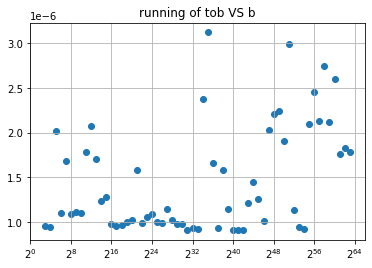
\includegraphics[scale=0.5]{images/simulation.png}
        \caption{X-axis represents input b and Y-axis represents time in seconds. The time for executing our function is very small compared to the overhead added time. So the simulation results are not clear enough.}
        \label{simulation_1}
    \end{figure}
    \item Used C itself to store the time data into a \textit{'.dat '} file. 
    \begin{figure}[]
        \centering
        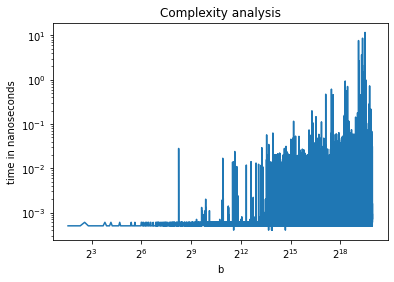
\includegraphics[scale=0.5]{images/simulation_2.png}
        \caption{Results seem more reasonable than previous attempt.}
        \label{simulation_2}
    \end{figure}
\end{enumerate}

\subsection{Implementation constraints}
\begin{itemize}
    \item Inputs are restricted by length of the array we are using to store binary representations, $y < 2^{length(array)}$, where $length(array)=20$.
    \item We are using \textit{int} data type in C to represent our integers so, $x^y < 2^{32}$.
\end{itemize}

\begin{figure}[]
    \centering
    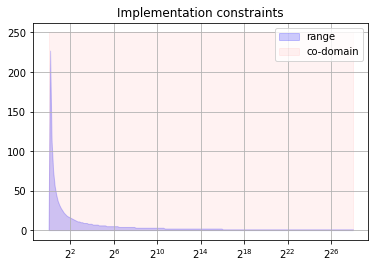
\includegraphics[scale=0.5]{images/constraints.png}
    \caption{Implementation restricts our range to the small purple shaded region.}
    \label{fig:constraints}
\end{figure}

\begin{itemize}
    \item We can improve those constraints at the cost of time complexity.
    \item Store large decimal number as a string.
    \item Treat individual character as a single digit number and take the remainder to the next character.
    \item This way we can perform division, multiplication and addition of the large number representated as string.
    \item Using that we convert that decimal string to binary string.
    \item Code for that can be found in \begin{lstlisting}
        https://github.com/Kkuntal990/C-DS/blob/main/Assignment1/codes/A1_4.cpp
    \end{lstlisting} of the repository.
    \item Time complexity : $\mathcal{O}(n)$, where n is the length of the large number. It is worse than previous logarithmic complexity.
    \item But we can convert integers containing more than 64 bits to their corresponding binary representation.
    \item Better range of our function can be obtained.
\end{itemize}


\end{document}